%Segunda Unidad
\begin{frame}{Teoremas preliminares}
\begin{block}{Teorema de Weierestrass}
Suponga que $f$ está definida y es continua en $[a, b]$. Para cada $\epsilon>0$, existe un polinomio $P(x)$, con la propiedad de que 
$$|f(x)-P(x)|<\epsilon, \quad \forall x \in [a, b]$$
\end{block}
\indent Los polinomios son ampliamente utilizados para la interpolación numérica porque:
\begin{itemize}
\item Aproximan de manera uniforme a las funciones conitnuas. 
\item Tienen derivadas e integrales fáciles de calcular. Además, sus integrales y derivadas también son polinomios. 
\end{itemize}
\indent Las principales limitaciones de los polinomios de Taylor son:
\begin{itemize}
\item Generalmente no ofrecen una buena aproximación en todo un intervalo, sino que la aproximación se concentra alrededor de $x_0$.
\item Aumentar el grado del polinomio de Taylor no necesariamente brindará una mejor aproximación.   
\item No utilizan más que un único punto para definir el polonomio.  
\end{itemize}
\end{frame}
%===========================
\begin{frame}{Limitaciones de los polinomios de Taylor para la interpolación}
\indent Debido a las limitaciones expuestas, los polinomios de Taylor se usan principalmente para:
\begin{enumerate}
\item Derivación de otros métodos numéricos, como el método de diferencias finitas.
\item Estimación del error
\end{enumerate}
\end{frame}

%===========================
\label{RetornoPolinomioLagrange}
\begin{frame}{Polinomio interpolante de Lagrange}
\begin{block}{Teorema: polinomios de Lagrange}
\indent Si $f$ es una funcion definida en los diferentes valores $\{x_0,\cdots, x_n\}$, entonces existe un único polinomio $P(x)$ de grado a lo más $n$, con la propiedad:
$$f(x_k)=P(x_k)\quad k=0, 1, \dots, n$$
El polinomio $P(x)$ se define como sigue:
\begin{align*}
P(x)&=\sum_{k=0}^{n}f(x_k)L_{n,k}(x)=f(x_0)L_{n,0}+\cdots+f(x_n)L_{n,n}
\end{align*}
donde
$$L_{n,k}=\frac{(x-x_0)(x-x_1)\dots(x-x_{k+1})(x-x_{k+1})\dots (x-x_n)}{(x_k-x_0)(x_k-x_1)\dots(x_k-x_{k+1})(x_k-x_{k+1})\dots (x_k-x_n)}$$
\end{block}
\end{frame}
%===========================
\begin{frame}
\begin{block}{Término del error del polinomio de Lagrange}
Suponga que $x_0, x_1, \dots, x_n$ son números distintintos en el intervalo $[a,b]$ y que $f \in C^{n+1}[a,b]$. Entonces, para cada x en $[a,b]$ existe in número $\xi(x)$ en $(a,b)$ con 
$$f(x)=P(x)+\frac{f^{(n+1)}(\xi(x))}{(n+1)!}(x-x_0)(x-x_1)\dots (x-x_n)$$
donde $P(x)$ es el polinomio interpolante de Lagrange.
\end{block}
\hyperlink{PolinomioLagrange}{\textcolor{cyan}{Enlace a ejercicio.}}
\end{frame}
\begin{frame}[allowframebreaks]{Interpolación, Spline Cúbicos}
\indent Considere el siguiente ajuste polinomial:
\begin{figure}[H]
\begin{center}
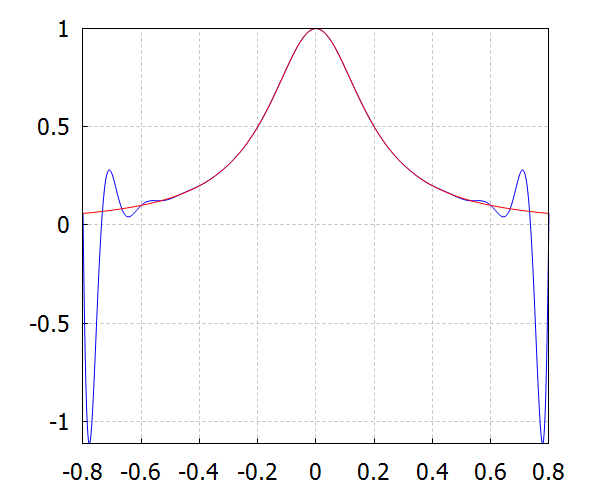
\includegraphics[scale=0.7]{Imagen21}
\end{center}
\caption{En la figura se observa la interpolación por polinomios de Lagrange para $f(x)=\dfrac{1}{1+25x^2}$ para $x\in[-1,1]$ con 30 puntos equidistante comenzando en -1 y finalizando en 1.}
\end{figure}
\indent El ejemplo anterior demuestra que los polinomios de alto orden (en el ejemplo de la figura tendríamos un polinomio de orden 31)  pueden oscilar erráticamente. Evidentemente esta característica es indeseable en muchas situaciones; en este apartado se mostrará una técnica que puede evitar este problema siempre con la idea de hacer un ajuste polinomial. \\
\indent Los ingredientes para construir un \textbf{spline} (esta palabra no tiene traducción al español, su significado es "larga tira flexible") \textbf{cúbico interpolante} $S$ de alguna función $f$ se basan en las siguiente consideraciones:
\begin{itemize}
\item Una función $f$ de variable real definida en el intervalo $[a,b]$.
\item Una partición del intervalo $[a,b]$; $a=x_0<x_1<\cdots<x_n=b$.
\item $S(x)$ restringido a $[x_j,x_{j+1}]$ es un polinomio cúbico para cada $j=0,\cdots, n-1$. A esta parte se le denota por $S_j(x)$.
\item $S_j(x_j)=f(x_j)$ y $S_{j}(x_{j+1})=f(x_{j+1})$ para cada $j=0,\cdots, n-1$.
\item $S'_{j+1}(x_{j+1})=S'_{j}(x_{j+1})$ para cada $j=0,\cdots, n-2$.
\item $S''_{j+1}(x_{j+1})=S''_{j}(x_{j+1})$ para cada $j=0,\cdots, n-2$.
\item Si $S''(x_0)=S''(x_n)=0$ se dice que es un \textbf{Spline de frontera natural}. Si $S'(x_0)=f'(x_0)$ y $S'(x_n)=f'(x_n)$ se dice que es un \textbf{Spline con frontera sujeta}. 
\end{itemize}
\begin{figure}
\begin{center}
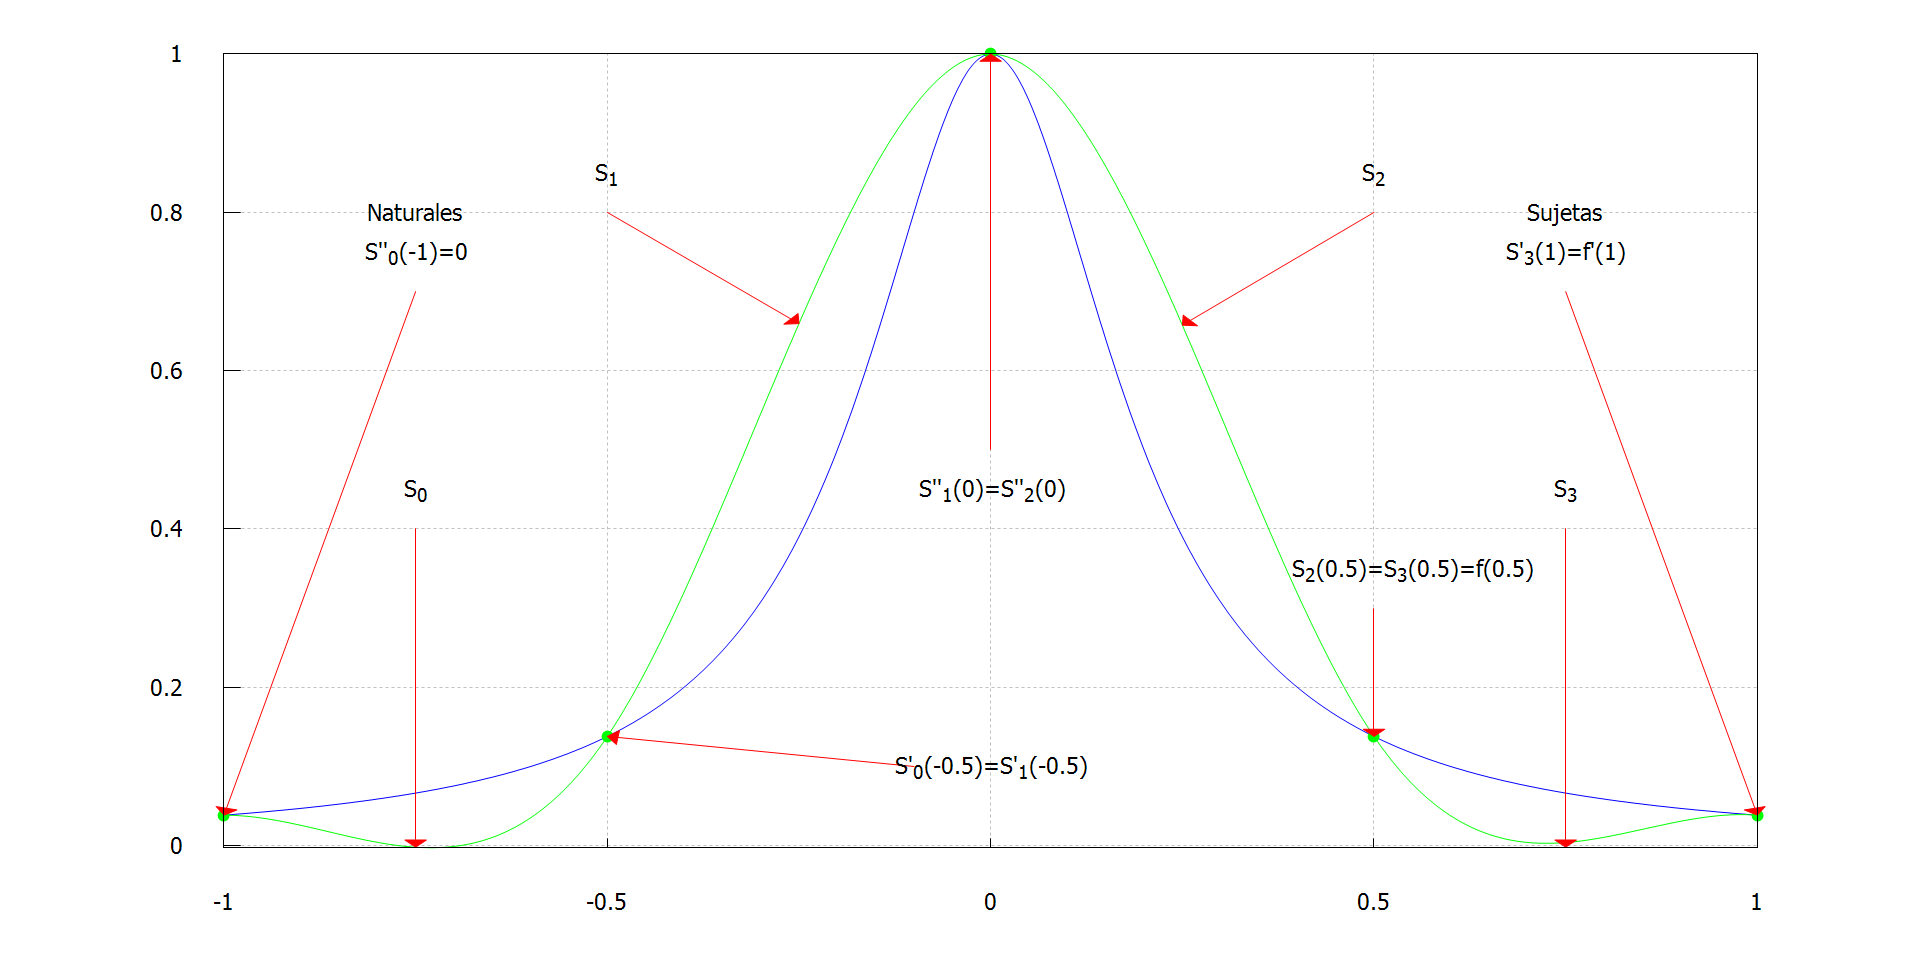
\includegraphics[scale=0.4]{Imagen22}
\end{center}
\caption{Aquí se muestran algunas condiciones de los spline. La función que se ve arriba en azul es $f(x)=\dfrac{1}{1+25x^2}$. En verde se observan los splines cúbicos.}
\end{figure}
\begin{block}{Fórmulas de recurrencia para los Splines Cúbicos}
\small
\indent Definanse los Splines Cúbicos de la función $f$ definida en $[x_0,x_n]$:
\begin{center}
$S(x)=S_j(x)\equiv a_j+b_j(x-x_j)+c_j(x-x_j)^2+d_j(x-x_j)^3$\\ para $x\in[x_j,x_{j+1}]$ donde $j=0,\cdots, n-1$.
\end{center}
\indent Por comodidad definanse los siguientes elementos:
\begin{center}
$a_n\equiv f(x_n)$, $b_n\equiv f'(x_n)$, $c_n\equiv f''(x_n)/2$, $h_j\equiv x_{j+1}-x_j$, $j=0,\cdots, n-1$.
\end{center}
\indent Las siguientes ecuaciones de recurrencia deben ser verificadas para que los $S_j$ cumplan con las condiciones de un Spline Cúbico.
\begin{enumerate}
\item $a_j\equiv f(x_j)$ para $j=0,\cdots, n-1$.
\item $a_j+b_jh_j+c_jh_j^2+d_jh_j^3=a_{j+1}$ para $j=0,\cdots, n-1$.
\item $b_j+2c_jh_j+3d_jh_j^2=b_{j+1}$ para $j=0,\cdots, n-1$.
\item $c_j+3d_jh_j=c_{j+1}$ para $j=0,\cdots, n-1$.
\item $\dfrac{3}{h_j}(a_{j+1}-a_j)-\dfrac{3}{h_{j-1}}(a_j-a_{j-1})=h_{j-1}c_{j-1}+2(h_{j-1}+h_j)c_j+h_jc_{j+1}$ para $j=1,\cdots, n-1$.
\end{enumerate}
\end{block}
\indent Las ecuaciones en el numeral 5 permiten resolver para los $\{c_j\}$; luego en el numeral 4 se pueden resolver los $\{d_j\}$ y con el numeral 2 se pueden encontrar los $\{b_j\}$. Los $\{a_j\}$ son conocidos desde el principio y con ello se pueden encontrar los Splines Cúbicos. \\
\indent Si se recuerda, $c_j$ está definido para $j=0,\cdots n$. Entonces es necesario encontrar $n+1$ valores. La ecuación en el numeral 5 solo provee de $n-1$ ecuaciones; por lo tanto faltan dos ecuaciones más que se podrán obtener de considerar las condiciones en la frontera (naturales o fijas). 
\end{frame}
\begin{frame}[allowframebreaks]{Mínimos cuadrados}
Considere el siguiente conjunto de datos $\{(x_i,y_i)\}_{i=1}^{N}$ asociados:
\begin{displaymath}
\begin{bmatrix}
1&2&3&4&5&6&7&8&9&10\\
\downarrow &\downarrow &\downarrow &\downarrow &\downarrow &\downarrow &\downarrow &\downarrow &\downarrow &\downarrow\\
3&5&9&11&15&17&20&24&26&29
\end{bmatrix}
\end{displaymath}
Abajo se aprecian los pares ordenados correspondientes a cada par asociado:
\begin{figure}[H]
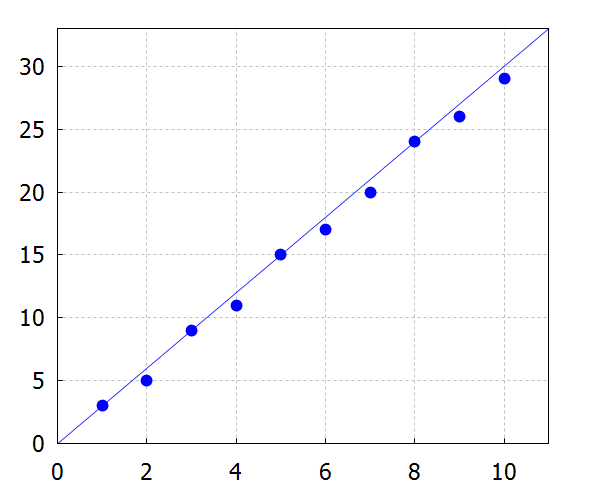
\includegraphics[scale=0.55]{Imagen2}
\caption{Recta de aproximación a los pares ordenados.}
\end{figure}
\indent El objetivo consiste en determinar la recta $Y=a_1X+a_0$ que mejor modele al conjunto de datos asociados.\\
\indent Existen algunos enfoques para encontrar esta recta:
\begin{block}{Problema Minimax}
\centering $\displaystyle \min_{a_0,a_1}\max_{1\leq i\leq 10}|y_i-(a_1x_i-a_0)|$
\end{block}
\begin{block}{Problema de desviación absoluta}
\centering $\displaystyle \min_{a_0,a_1}\sum_{i=1}^{10}|y_i-(a_1x_i-a_0)|$
\end{block}
\begin{block}{Problema de mínimos cuadrados}
\centering $\displaystyle \min_{a_0,a_1}\sum_{i=1}^{10}|y_i-(a_1x_i-a_0)|^2=\displaystyle \min_{a_0,a_1}\sum_{i=1}^{10}(y_i-(a_1x_i-a_0))^2$
\end{block}
\end{frame}
\begin{frame}{Deducción del método de mínimos cuadrados}
Defina los siguientes vectores:
$$X=[x_1,\cdots,x_n]^T$$
$$Y=[y_1,\cdots,y_n]^T$$
$$U=[1,\cdots,1]^T$$
Entonces podemos pensar en el problema de ajuste de la siguiente manera: Deseamos encontrar $a_0$ y $a_1$ tales que
$$a_1X+a_0U=Y$$
De forma matricial esto sería:
\begin{displaymath}
(X|U)
\left(
\begin{array}{c}
a_1\\
a_0
\end{array}
\right)=Y
\end{displaymath}
\end{frame}
\begin{frame}{Deducción del método de mínimos cuadrados}
Si ahora se multiplica por la transpuesta de la primer matriz, se obtine:
\begin{displaymath}
\left(
\begin{array}{c}
X^T\\
U^T
\end{array}
\right)
(X|U)
\left(
\begin{array}{c}
a_1\\
a_0
\end{array}
\right)=
\left(
\begin{array}{c}
X^T\\
U^T
\end{array}
\right)
Y
\end{displaymath}
Esto es equivalente a lo siguiente:
\begin{displaymath}
\left(
\begin{array}{cc}
X^TX &X^TU\\
U^TX & U^TU
\end{array}
\right)
\left(
\begin{array}{c}
a_1\\
a_0
\end{array}
\right)=
\left(
\begin{array}{c}
X^TY\\
U^TY
\end{array}
\right)
\end{displaymath}
Como se puede apreciar, resolviendo este sistema podemos encontrar las soluciones para los coeficientes de la regresión lineal.
\end{frame}
\begin{frame}{Generalización a ajustes de tipo polinomial.}
Ahora considere le problema siguiente: Se desan encontrar los valores $[a_m,a_{m-1},\cdots,a_0]$ de manera tal que:
$$a_mX^m+\cdots+a_1X+a_0U=Y$$
Donde $X^k=[x_1^k,\cdots,x_n^k]^T$. Nuevamente esto se puede escribir como el siguiente sistema:
\textcolor{red}{
\begin{displaymath}
(X^m|X^{m-1}|\cdots X|U)
\left(
\begin{array}{c}
a_m\\
\vdots\\
a_0
\end{array}
\right)=Y
\end{displaymath}
}
Multiplicando por la transpuesta...
\end{frame}
\begin{frame}{Generalización de ajuste  de tipo polinomial}
\begin{displaymath}
\left(
\begin{array}{c}
(X^m)^T\\
\vdots\\
(X)^T\\
U^T
\end{array}
\right)
(X^m|X^{m-1}|\cdots X|U)
\left(
\begin{array}{c}
a_m\\
\vdots\\
a_0
\end{array}
\right)=
\left(
\begin{array}{c}
(X^m)^T\\
\vdots\\
(X)^T\\
U^T
\end{array}
\right)
Y
\end{displaymath}
Lo que termina siendo equivalente a resolver el sistema:
\begin{displaymath}
\left(
\begin{array}{cccc}
(X^m)^TX^m & (X^m)^TX^{m-1} &\hdots & (X^m)^TU\\
\vdots&\vdots &&\vdots\\
(X)^TX^m&(X)^TX^{m-1}&\hdots &(X)^TU\\
U^TX^m&U^TX^{m-1}&\hdots &U^TU
\end{array}
\right)
\left(
\begin{array}{c}
a_m\\
\vdots\\
a_0
\end{array}
\right)=
\left(
\begin{array}{c}
(X^m)^TY\\
\vdots\\
(X)^TY\\
U^TY
\end{array}
\right)
\end{displaymath}
\end{frame}